% --- Depth Anything and SuperGlue ---
% --- Depth Estimation: Depth Anything ---
\begin{frame}{Depth Estimation Foundation Model: Depth Anything}
  \begin{itemize}
    \item Foundation model for single image depth estimation.
    \item Trained with a large-scale teacher-student pipeline:
      \begin{itemize}
        \item $\sim$1.5M labeled images + $\sim$62M unlabeled images
      \end{itemize}
    \item Encoder priors from DINOv2 improve cross-domain geometric understanding.
    \item Robust transfer across indoor/outdoor domains with limited task-specific supervision.    
    \item Applications:
      \begin{itemize}
        \item Robotics and autonomous driving
        \item Virtual/augmented reality
        \item 3D scene understanding and reconstruction
      \end{itemize}
  \end{itemize}
\end{frame}

\begin{frame}{How Depth Anything Works}
  \begin{itemize}\footnotesize
    \item \textbf{Teacher--student pipeline} on labeled depth plus large-scale unlabeled RGB: pseudo-labels from the teacher.
    \item DINOv2-style encoder + prediction head maps RGB to per-pixel depth.
    \item Outputs dense depth maps that transfer to segmentation and other geometric downstream tasks.
  \end{itemize}
  \centering
  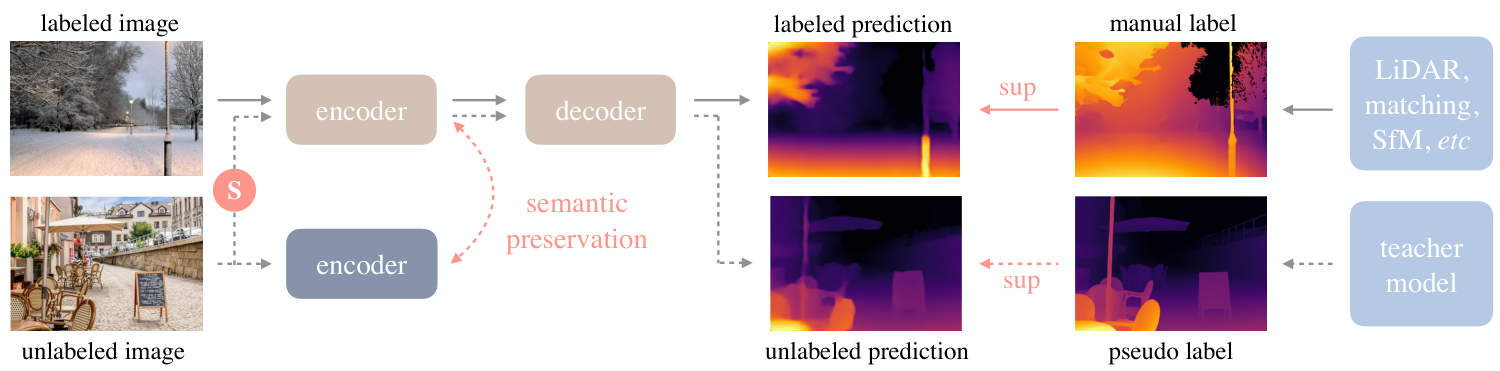
\includegraphics[width=0.95\textwidth]{assets/New-Lecture_Foundation_models/depth_anything_cvpr2024_fig2_pipeline.png}\\[0.15em]
  {\scriptsize Yang et al., ``Depth Anything,'' CVPR 2024 (\href{https://openaccess.thecvf.com/content/CVPR2024/papers/Yang_Depth_Anything_Unleashing_the_Power_of_Large-Scale_Unlabeled_Data_CVPR_2024_paper.pdf}{OpenAccess}).}
\end{frame}

% % --- Keypoint Detection: SuperGlue ---
\begin{frame}{SuperGlue: Foundation model for Keypoint Detection}
  \begin{itemize}
    \item Combines graph neural networks and attention to find matches between sets of keypoints in different images.
    \item Generalizes across scenes and keypoint detector types.
    \item Applications: Visual localization and mapping, 3D reconstruction, Object pose estimation.
  \end{itemize}
\end{frame}

\begin{frame}{SuperGlue: Model Architecture}
  \begin{columns}[T,onlytextwidth]
    \begin{column}{0.44\textwidth}
      \begin{itemize}\scriptsize
            \item Two main components: an attentional graph neural network (GNN) and an optimal matching layer.
            \item GNN uses keypoint encoder to combine each keypoint's position and visual descriptor into single vector.
            \item Alternating self-attention and cross-attention layers create powerful feature representations.
            \item The optimal matching layer builds an $M\times N$ score matrix between keypoints of both images, appends additional rows/columns (``dustbins'') for potential unmatched keypoints.
            \item Uses Sinkhorn algorithm for $T$ iterations to find optimal partial matching assignment.
          \end{itemize}
    \end{column}
    \begin{column}{0.54\textwidth}
      \centering
      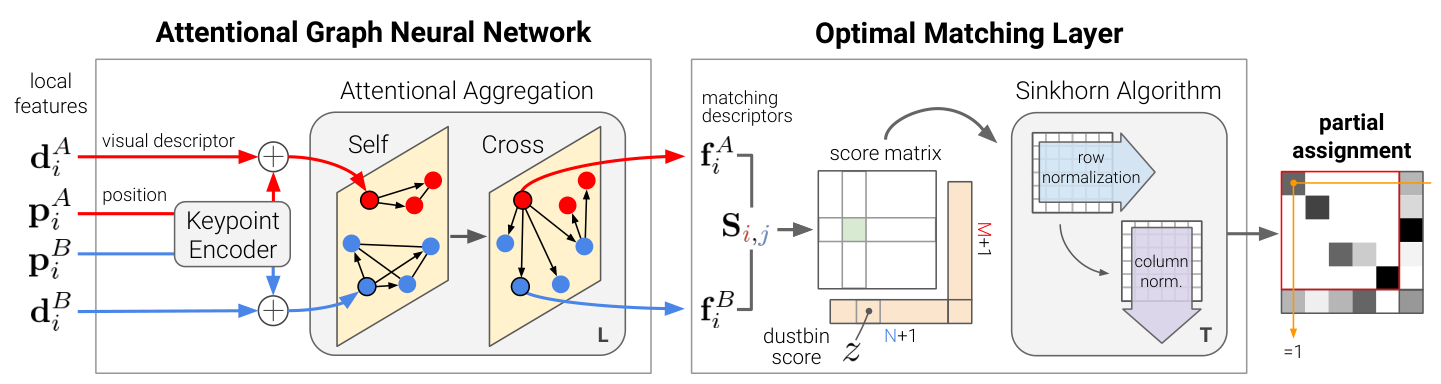
\includegraphics[width=\linewidth]{assets/New-Lecture_Foundation_models/superglue_cvpr2020_fig3_architecture.png}\\[0.2em]
      {\scriptsize Sarlin et al., ``SuperGlue: Learning Feature Matching with Graph Neural Networks,'' CVPR 2020 (\href{https://openaccess.thecvf.com/content_CVPR_2020/papers/Sarlin_SuperGlue_Learning_Feature_Matching_With_Graph_Neural_Networks_CVPR_2020_paper.pdf}{OpenAccess}).}
    \end{column}
  \end{columns}
\end{frame}
